\chapter{Unmanned Aircraft System Overview}\label{ch:uas}

Unmanned Aircraft System, UAS, is the hardware responsible for keeping the connection between the GS and the UA. However, when the distance between these two elements increases, the quality of the signal that is received and sent by both antennas is reduced. Therefore, it is essential to have the proper physical infrastuctures to be able to detect both strong and weak signals. These infrastuctures constitute the hardware and they cover every element connected with the vehicle, in the air, and the ground station, on the ground.

%However, increasing of the distance will reduce the quality of the signal that is received and sent by both antennas. In order to keep the communication, it is essential to have the proper physical infrastuctures to be able to detect both strong and weak signals. These infrastuctures constitute the hardware and they cover every element connected with the vehicle, in the air, and the ground station, on the ground. The previous description of the system as a whole constitutes the Unmanned Aerial System, UAS.

The structure of the UAS illustrated in Figure \ref{fig:uas} can be decomposed in the following elements:
\begin{itemize}
	\item Unmanned Aircraft (UA)
	\item Ground Station (GS)
	\item Antennas
	\item Mission sensors
\end{itemize}

\begin{figure}[H]
	\centering
	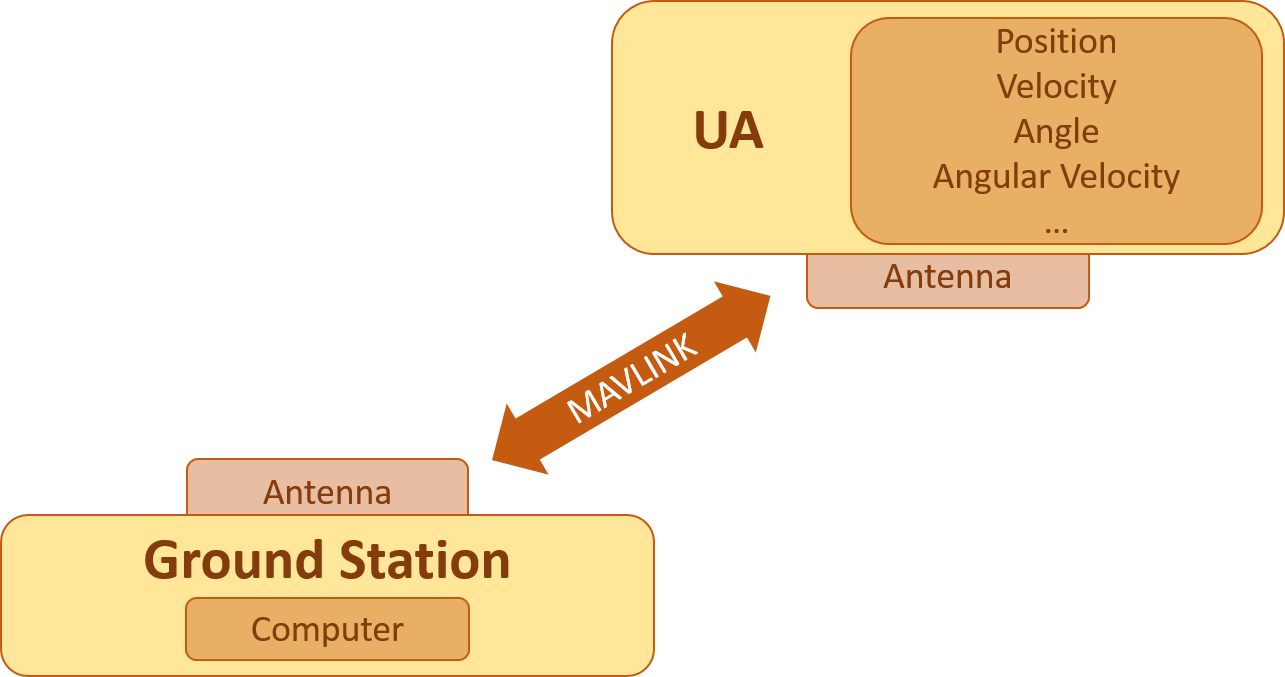
\includegraphics[scale=0.4]{figures/uas.png}
	\caption{Unmanned Aircraft System (UAS) Diagram}
	\label{fig:uas}
\end{figure}

%In order to have some bounds of the system we can have a look at the drone performances:
%\begin{itemize}
%	\item 50 km/h - stability at high speeds 
%	\item 40 minutes - battery autonomy (30 minutes with payload)
%	\item 2400 m - maximum flight altitude (higher if take off from mountain site)
%	\item 50 km - maximum radio communication (with directional antennas)
%	\item under 1 m - absolute positioning of X-Y GPS
%	\item GPS return-to Home (automatically activates when radio link is lost)
%\end{itemize}


